\documentclass[12pt]{article}
\usepackage{amsmath}
\usepackage{amsfonts}
\usepackage{url}
\usepackage{float}
\usepackage{multicol}
\usepackage{chemformula}
\usepackage{hyperref}
\hypersetup{
	colorlinks=true,
	linkcolor=blue,
	filecolor=magenta,      
	urlcolor=blue,
	citecolor=blue
}
\usepackage{graphicx}
\usepackage{subcaption}
\usepackage{url}
\usepackage{siunitx}
\usepackage{listings}
\usepackage{color} %red, green, blue, yellow, cyan, magenta, black, white
\definecolor{mygreen}{RGB}{28,172,0} % color values Red, Green, Blue
\definecolor{mylilas}{RGB}{170,55,241}
\setlength{\oddsidemargin}{0in}
\setlength{\evensidemargin}{0in}
\setlength{\textheight}{9in}
\setlength{\textwidth}{6.5in}
\setlength{\topmargin}{-0.5in}

\usepackage[backend=biber,sorting=none,style=nature]{biblatex}
\addbibresource{biblio.bib}

\DeclareSIUnit\atm{atm}

\title{\bf Assignment 3 \\[2ex] 
	\rm\normalsize Electronic Structure Theory}
\date{\today}
\author{\bf Declan Mathews [s1610357][B103565]}

\begin{document}
	\maketitle
	
\section*{Phonon Convergence}

N.B.  The grids discussed are all isotropic with the DFPT q-point grid as (Nq Nq Nq) and the post-processing q-point grid as (Nk Nk Nk) where Nq and Nk are positive integers. When a 'larger' grid size is referred to, this means that Nq or Nk is larger, and so a more fine grid with more q-points is used in the calculations.

\subsection*{Density of States (DOS) convergence}

The convergence of the DOS graph was studied for varying grids in both the DFPT calculation and the post-processing step. The two main ways to determine this were by eye and by plotting a heatmap of the difference from a 'converged' state (taken as the result for the finest calulated grid which was with Nk and Nq equal to 14). Figure \ref{fig:ppdos} shows the convergence when the post-processing grid is varied and the DFPT grid is kept constant and Figure \ref{fig:dfptdos} shows the convergence for when the DFPT grid is varied instead. Finally, the heatmap in Figure \ref{fig:matdos} shows the quantitative difference. As the finding the difference at each calculated frequency point produces a list, this can be treated as a vector and finding the magnitude of it produces a scalar to plot as the intensity. This isn't physically meaningful but is useful to produce a single value to represent the difference.

\begin{figure}[!htpb]
	\centering
	\begin{subfigure}{0.5\textwidth}
	\centering
	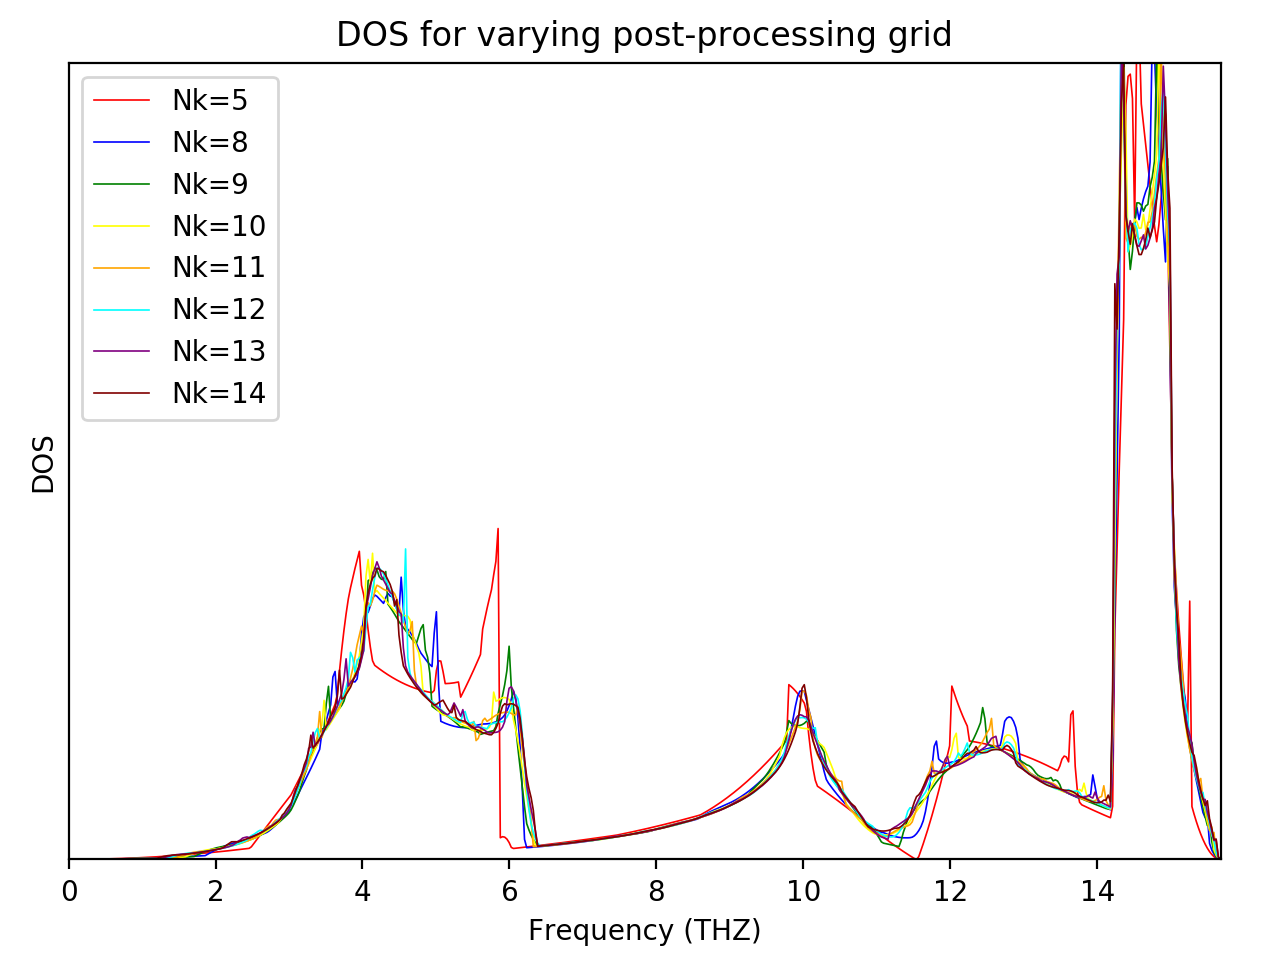
\includegraphics[width=8cm]{../Figures/dos_pp_vary.png}
	\subcaption{}
	\label{fig:ppdoswhole}
	\end{subfigure}%
	\begin{subfigure}{0.5\textwidth}
	\centering
	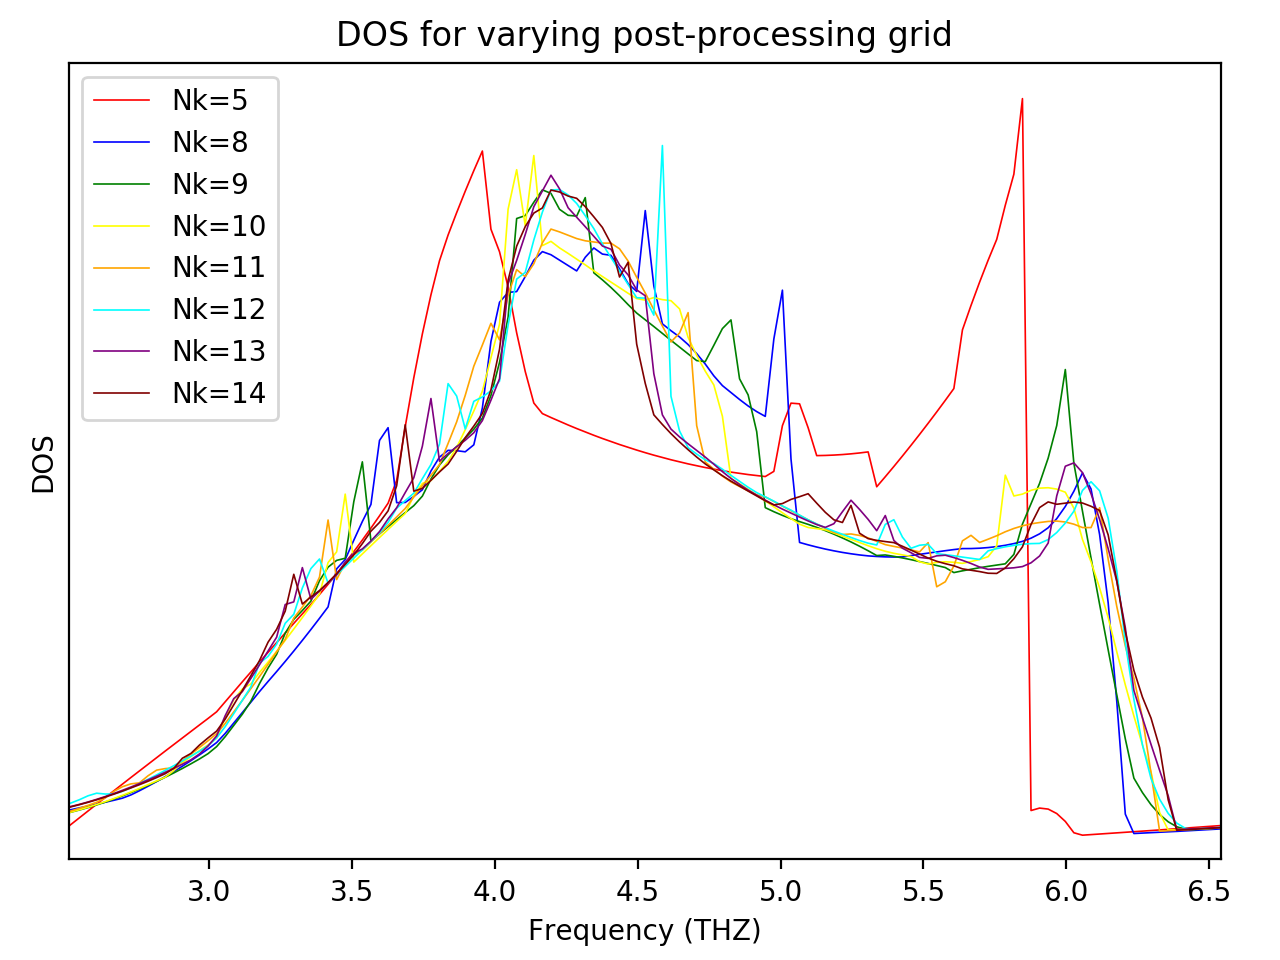
\includegraphics[width=8cm]{../Figures/dos_pp_vary_zoom.png}
	\subcaption{}
	\label{fig:ppdoszoom}
\end{subfigure}%
\caption{The DOS of Silicon for verying post-processing grid while the DFPT grid is kept at (11, 11, 11). The image on the right is a magnification of the left image to show the variation in more detail.}
\label{fig:ppdos}
\end{figure}

\begin{figure}[!htpb]
	\begin{subfigure}{0.5\textwidth}
	\centering
	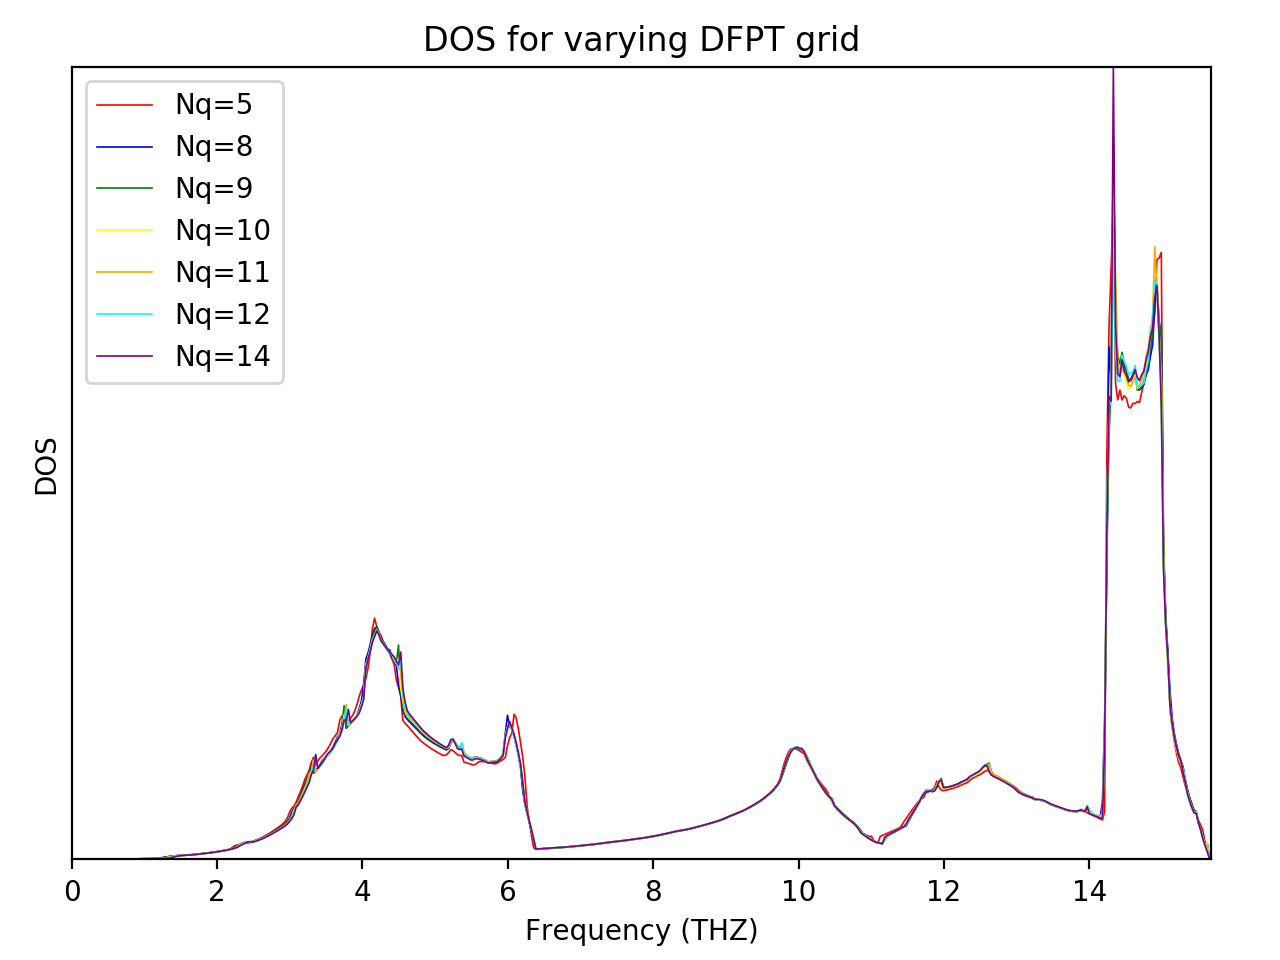
\includegraphics[width=8cm]{../Figures/dos_dfpt_vary.png}
	\subcaption{}
	\label{fig:dfptdoswhole}
\end{subfigure}%
	\begin{subfigure}{0.5\textwidth}
	\centering
	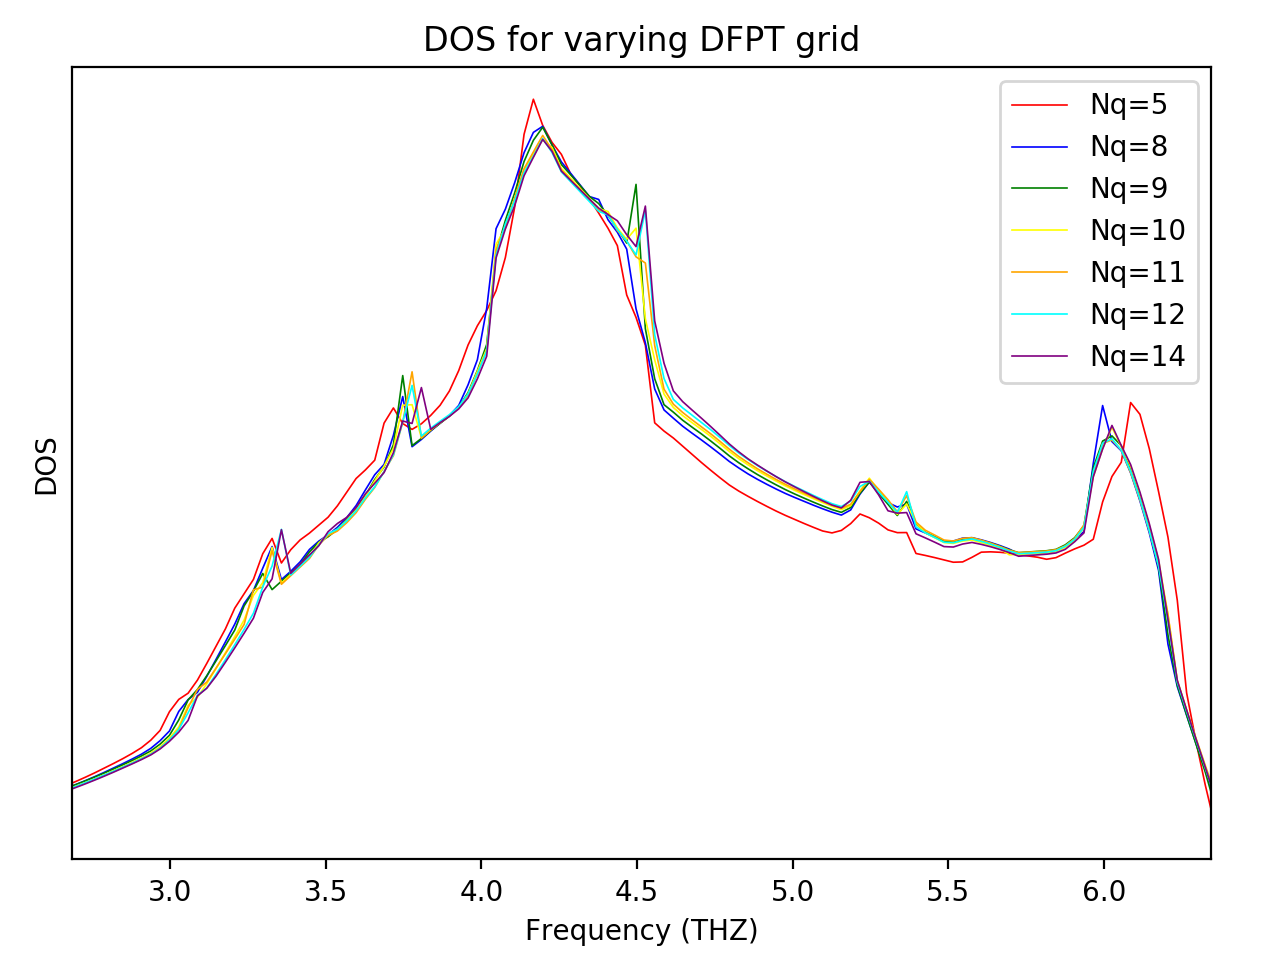
\includegraphics[width=8cm]{../Figures/dos_dfpt_vary_zoom.png}
	\subcaption{}
	\label{fig:dfptdoszoom}
\end{subfigure}%
\caption{The DOS of Silicon for varying DFPT grid while the post-processing grid is kept at (13, 13, 13). The image on the right is a magnification of the left image to show the variation in more detail.}
\label{fig:dfptdos}
\end{figure}

\begin{figure}[!htpb]
	\centering
	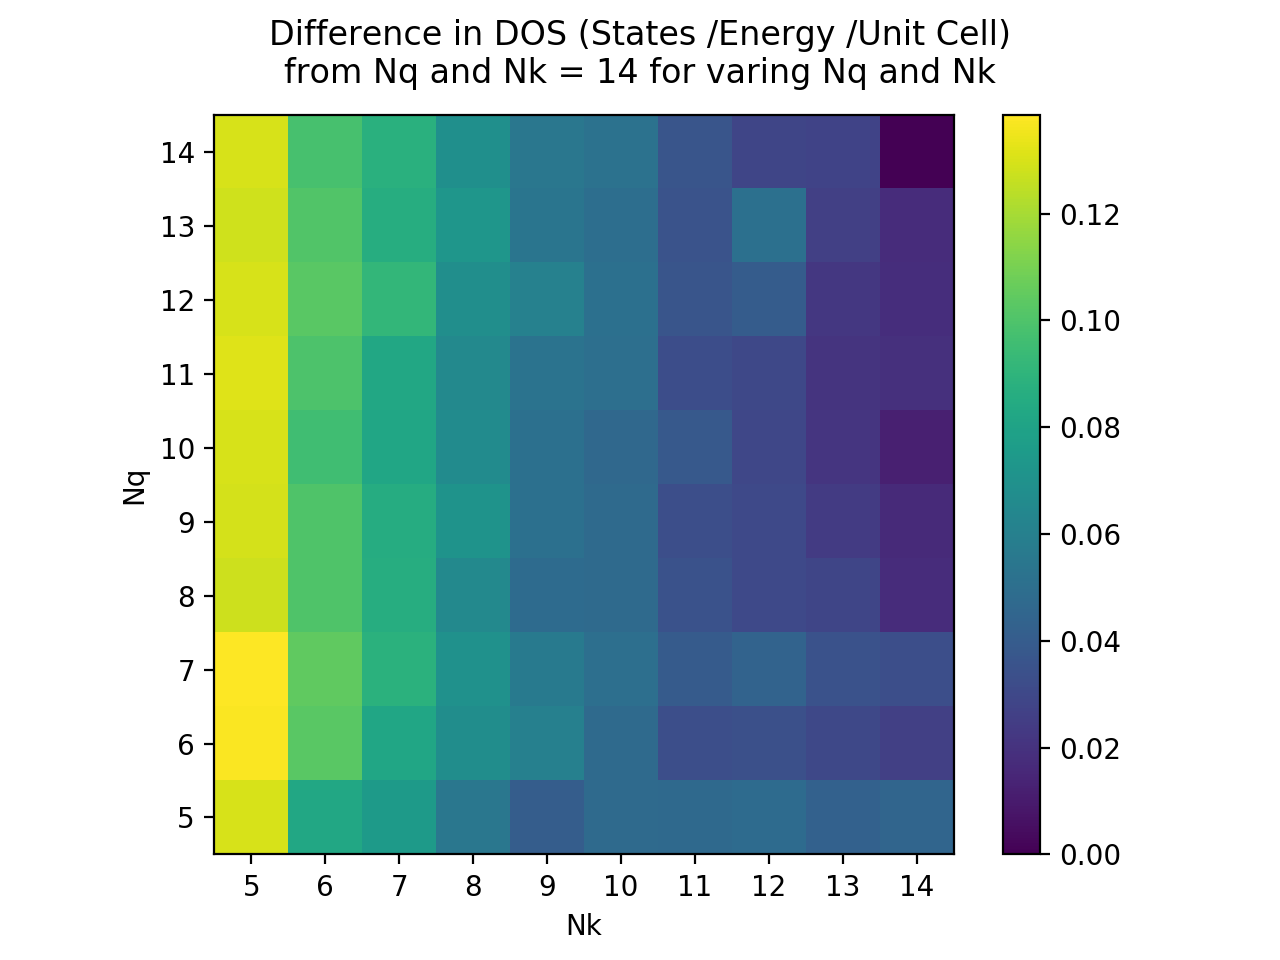
\includegraphics[width=12cm]{../Figures/mat_dos.png}
	\caption{The difference in the DOS of Silicon for DFPT grid of (Nq, Nq, Nq) and post-processing grid of (Nk, Nk, Nk) from the Nq=Nk=14 calculation. The Nk=Nq=14 state is considered the 'converged' state to compare to when determining a sufficient convergence without reaching this point to save computational expense.}
	\label{fig:matdos}
\end{figure}

\bigskip

\noindent The figures and heat map show that the post-processing grid has a larger impact on the convergence of the DOS. Both Figure \ref{fig:ppdos} and \ref{fig:dfptdos} show that increasing the value of Nk or Nq (and so creating a finer grid) produces a convergence towards the true DOS. The heat map in Figure \ref{fig:matdos} agrees with this results. The heat map clearly shows a larger change in the difference when moving along the x-axis (post-processing grid) compared to the y-axis (DFPT grid), indicating the larger impact of the post-processing grid size.  The heat map also shows a darker blue area in the top right, from about Nq=8 and Nk=11, where a better converged state is achieved, although with some noise due to only one run being carried out per site on the grid. Any state in this upper right corner could be argued for as being converged. Based on these results I would select Nq=11 and Nk=13, however, the dispersion convergence can also impact the choice of Nq.


\subsection*{Dispersion convergence}

The phonon dispersion also varies when the DFPT q-grid is varied. Figure \ref{fig:dfpt-big-band-vary} shows the variation for a very coarse grid with Nq = 4 compared with a much finer grid of Nq = 14. There is some distinct variation where the red lines can be seen, particularly near the $\Gamma$ point, but the difference is hard to distinguish, with the difficulty increasing as the unconverged Nq is increased. To qantitively study the difference, the average difference per dispersion band at each calculated point in the first Brillouin zone is plotted for varying Nq values from the 'converged' Nq=14 result in Figure \ref{fig:dfptband}.

\begin{figure}[!htpb]
	\centering
	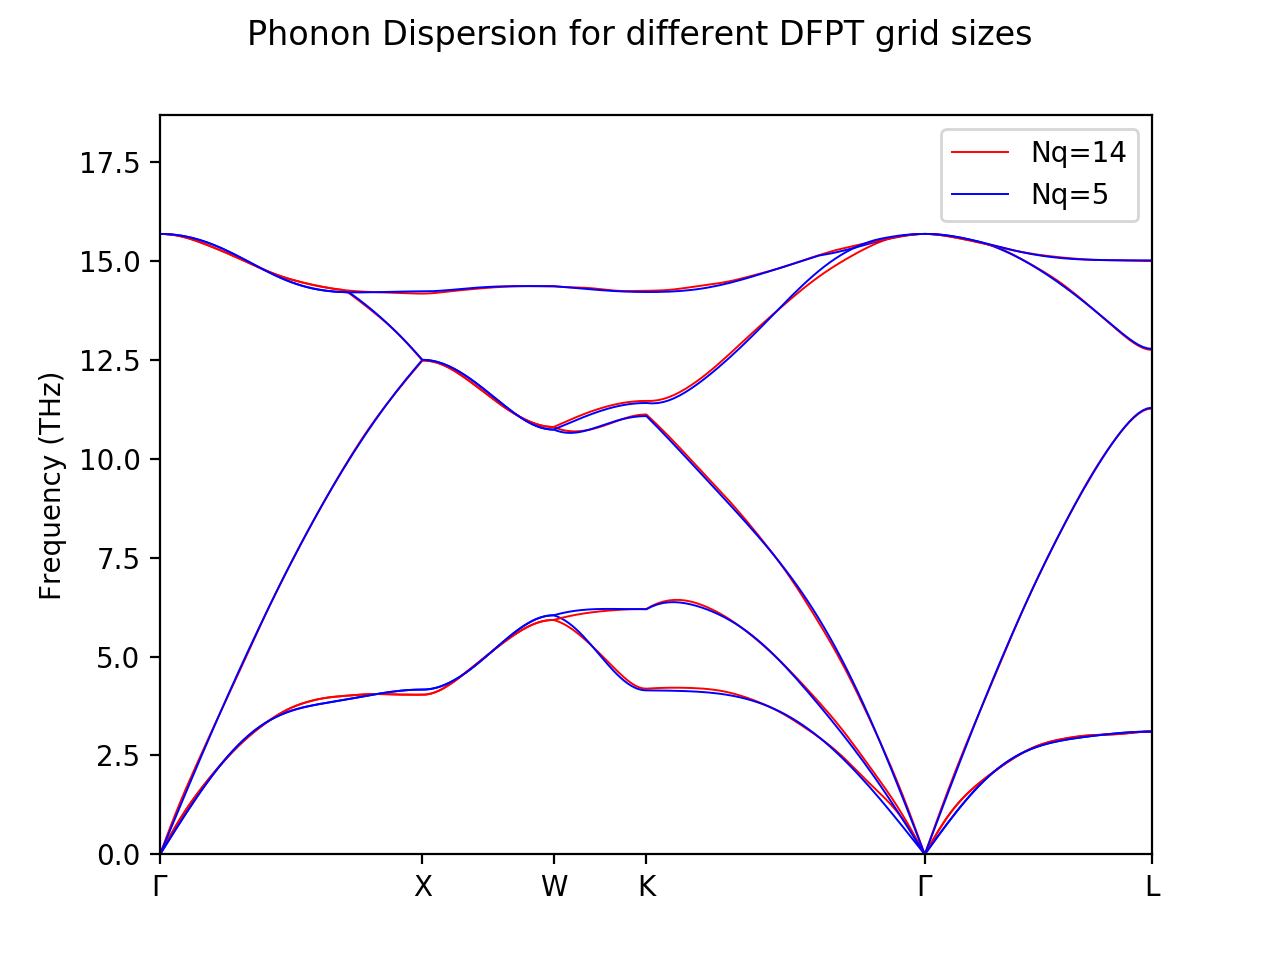
\includegraphics[width=12cm]{../Figures/disp_vary.png}
	\caption{The phonin dispersion graphs for Nq=14 and Nq=5 when Nk=10. The sections when the red line becomes visible is when the Nq=5 result deviates from the 'converged' result.}
	\label{fig:bandvary}
\end{figure}

\begin{figure}[!htpb]
	\begin{subfigure}{0.5\textwidth}
		\centering
		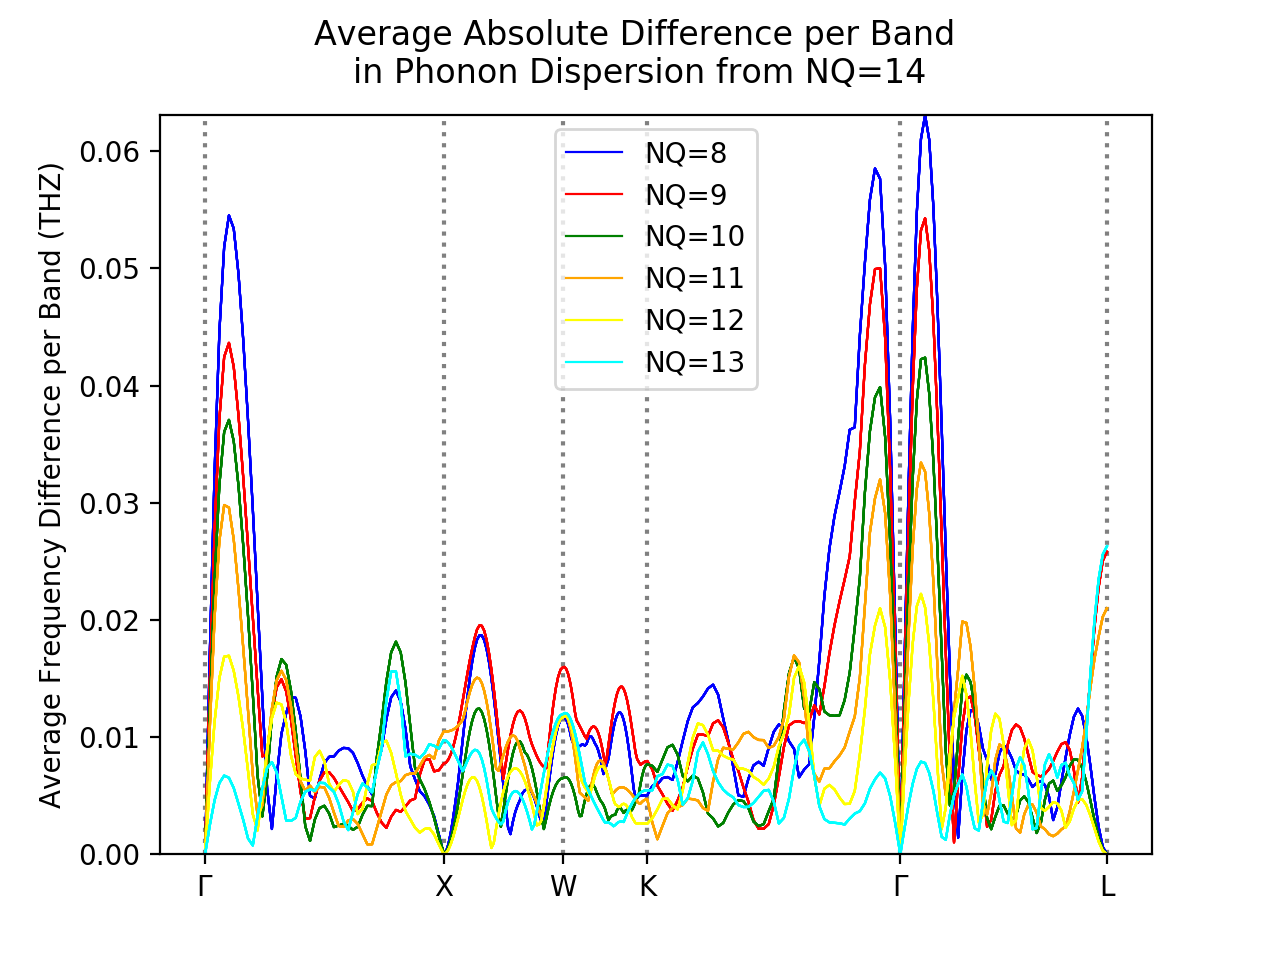
\includegraphics[width=8cm]{../Figures/disp_convergence.png}
		\subcaption{}
		\label{fig:dfptbandwhole}
	\end{subfigure}%
	\begin{subfigure}{0.5\textwidth}
		\centering
		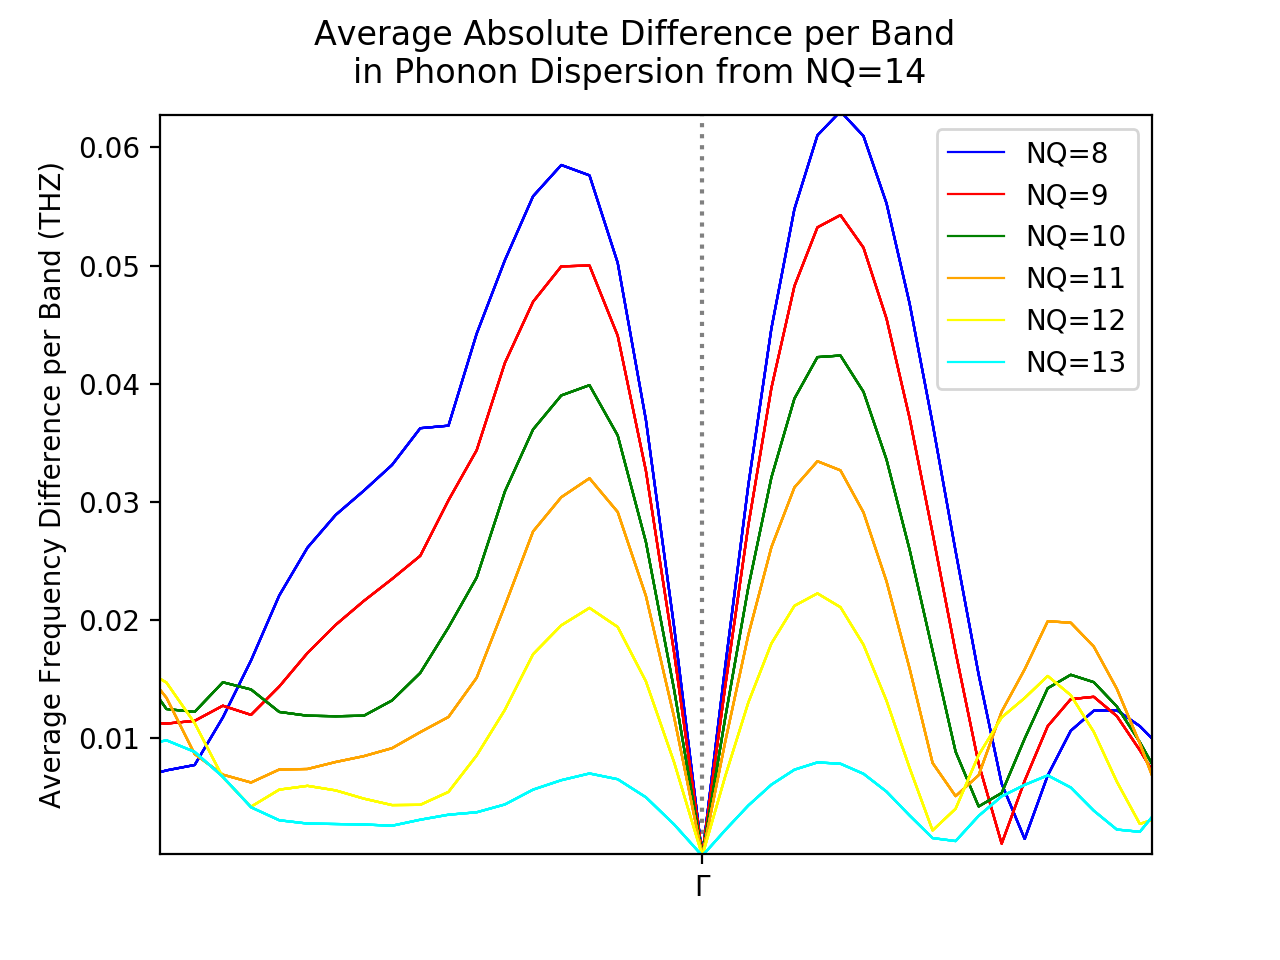
\includegraphics[width=8cm]{../Figures/disp_convergence_zoom.png}
		\subcaption{}
		\label{fig:dfptbandzoom}
	\end{subfigure}%
	\caption{The average difference per dispersion band at each calculated point in the first Brillouin zone for varying Nq but fixed Nk=10. The image on the right is a magnification of the left image to show the variation in more detail around the $\Gamma$ point.}
	\label{fig:dfptband}
\end{figure}

\bigskip

\noindent Figure \ref{fig:bandvary} shows clear differences in the phonon dispersions, particularly at the $\Gamma$ point. However, the differences are hard to distinguish by eye and so Figure \ref{fig:dfptband} shows the difference quantitively. The regions not near the $\Gamma$ point are also slightly unclear in this graph but by zooming in around the $\Gamma$ point a much clearer convergence can be seen. This is also the area with the largest difference compared to the 'converged' state and so gives a slightly better estimate for the level of convergence achieved. It shows that, as expected, the difference decreases as the number of grid points is increased. The convergence is small, as seen in \ref{fig:bandvary} by the small deviations. Independently, it is not clear where to select a cutoff in the convergence graphs in \ref{fig:dfptband}. However, when comparing with the cutoff values determined for the DOS we can see that the results indicate that Nq=11 is slightly more converged than lower values. Using the combination of these results the converged result is expected at Nq=11 and Nk=13.

\bigskip

\noindent It is worth noting that a lower Nq value is more desireable due to the significantly increasing computation cost with higher Nq values. Higher Nk values also increase the time but on a much smaller and negligible scale (to a realistic extent). This factors into the decision here slightly, as if deciding to choose between a slightly more converged Nq=12 rather than Nq=11, without losing much precision the lower value is more desireable. Also, during the analysis the grids were often plotted and studied by eye, to pick out any large spikes or anomalies that affected the shape or convergence. To some extent this is captured in the quantitive study, but is not explicitly shown here as this was done interactively via adding and removing lines in gnuplot to study the changes. This was done to confirm the results achieved here (successfully) and for understanding.

\bigskip

\noindent The final converged band structures for Nq = 11 and Nk = 13 are shown in Figure \ref{fig:band-dos}. The black points correspond to experimental data which will be discussed further in the next section.

\begin{figure}[!htpb]
	\centering
	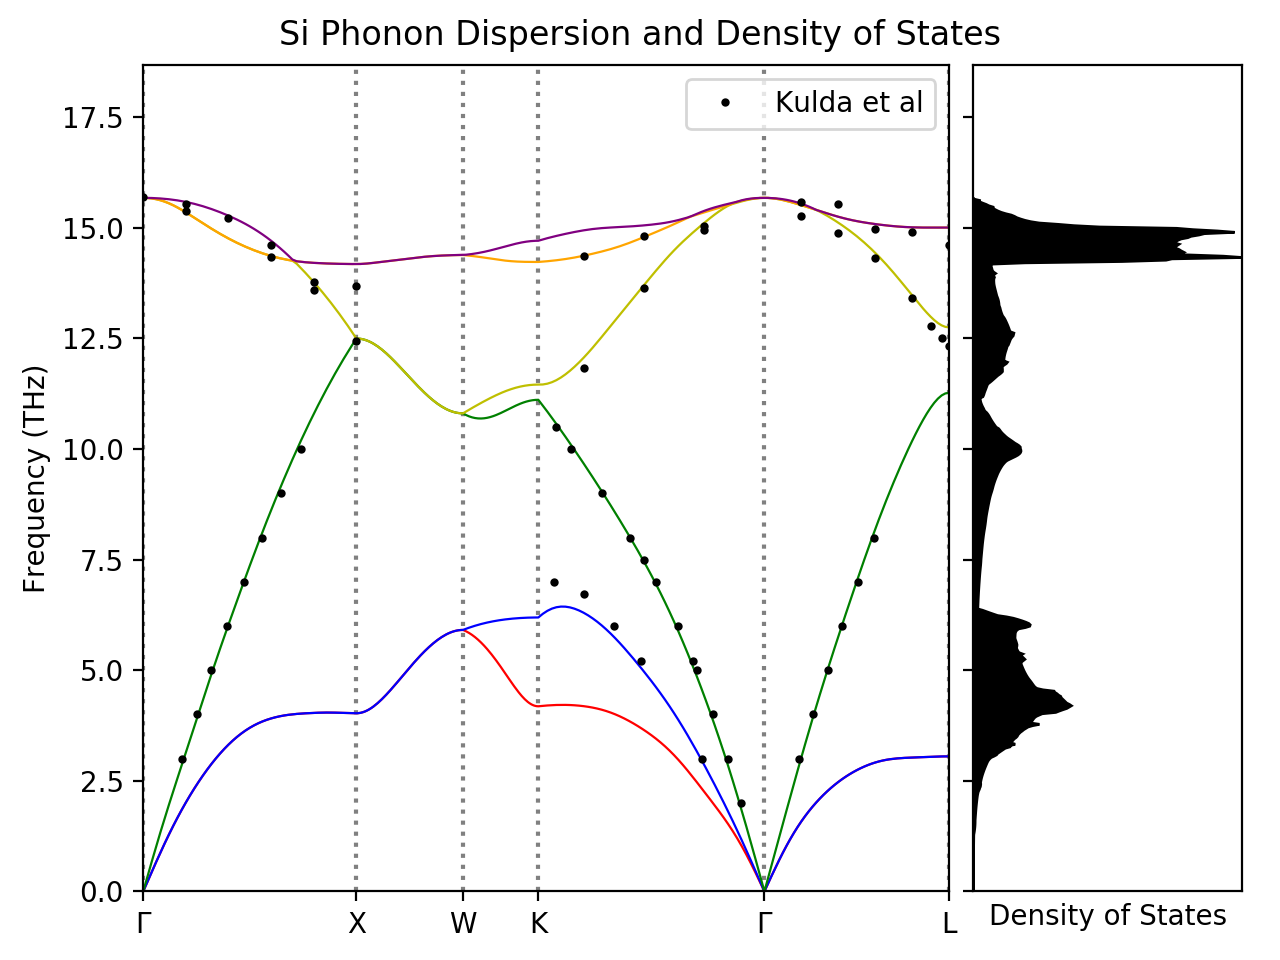
\includegraphics[width=12cm]{../Figures/si_disp_dos.png}
	\caption{Silicon phonon dispersion and DOS when Nk=13 and Nq=11. The black points are the experimental results\cite{Kulda}. }
	\label{fig:band-dos}
\end{figure}

\bigskip

\noindent The final results for the phonon dispersion and DOS of silicon in Figure \ref{fig:band-dos} agree well with each other. The dispersion has six bands, all at positive frequencies and with three acoustic and three optical as expected.

\clearpage	
\section*{Phonon Observables}

Using the first ten data points of the acoustic branches emerging from the gamma point, a linear fit was carried out to determine the gradient. Two of the bands overlap in this region and correspond to transverse speed of sound while the third band corresponds to the longitudinal speed of sound.
The results of the fit are shown in Table \ref{tab:c}. 

\bigskip

\begin{table}[!htpb]
	\centering
	\begin{tabular}{c|c|c|}
		\cline{2-3}
		& Experimental & This Study \\ \hline
		\multicolumn{1}{|c|}{Longitudinal (ms$^{-1}$)} & 8433         & 8609       \\ \hline
		\multicolumn{1}{|c|}{Transverse (ms$^{-1}$)}   & 5843         & 5625       \\ \hline
	\end{tabular}
\caption{The derived longitudinal and transverse speeds of sound in Silicon from the results in this study and the experimental results from \cite{sic}.}
\label{tab:c}
\end{table}

\bigskip

\noindent The comparison of the phonon dispersion to raman spectroscopy data\footnote{\label{ramandata}https://rruff.info/Silicon} is shown in Figure \ref{fig:raman}.

\begin{figure}[!htpb]
	\centering
	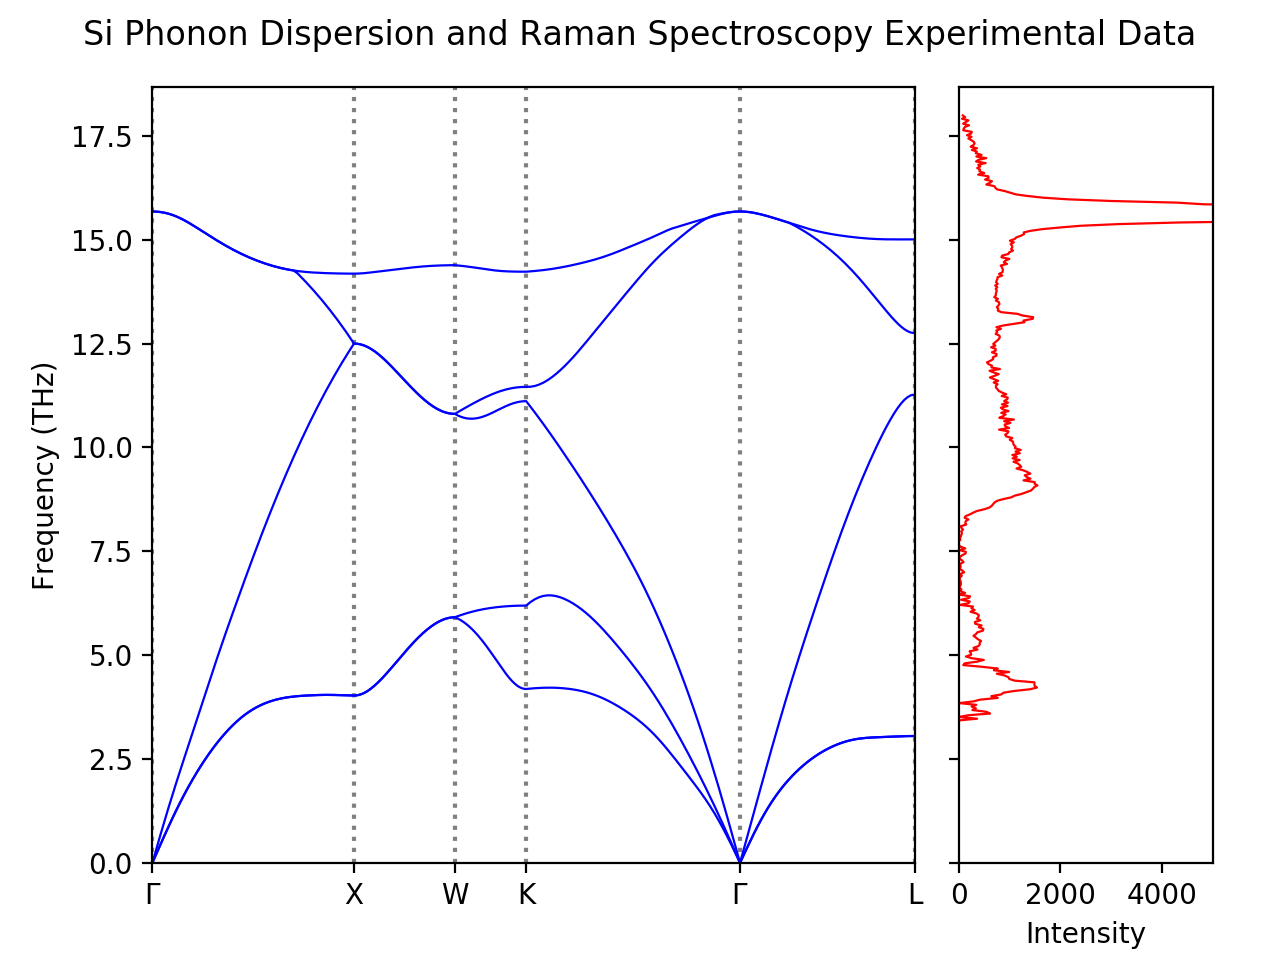
\includegraphics[width=12cm]{../Figures/raman.png}
	\caption{Silicon phonon dispersion when Nk=13 and Nq=11 and raman spectroscopy data from footnote \ref{ramandata}. The large peak at roughly 16 THz (or 520 cm$^{-1}$) is cut off to provide a clearer picture. }
	\label{fig:raman}
\end{figure}

\bigskip

\noindent The sound velocities of Si agree well with the experimental values. However, these values depend on the plane of measurement. Other studies have found the longitudinal velocity varying between 8433 and 9322 ms$^{-1}$ \cite{sicvary}, although this is still in good agreement with the derived result here. This can also be seen in the dispersion plot, as the transverse bands are degenerate between $\Gamma$ and X and also between $\Gamma$ and L, but not between K and $\Gamma$. This is due the plane of the direction between them. For the sound velocity results here the $\Gamma$-X data was used (the [100] plane).

The triply degenerate optical mode also corresponds very well with the raman spectroscopy data seen in Figure \ref{fig:raman}. Both the determined dispersion and the raman data plotted agree well with experimental results\cite{raman} quoting 520.5 cm$^{-1}$ (15.6 THz) for the large intensity peak at the triply degenerate optical mode. 

Finally, the neutron scattering results plotted on the dispersion data in Figure \ref{fig:band-dos} agrees well the calculated results here. There are notable differences, particularly in the optical modes and near the X point, but the overall trends are similar and the results near the $\Gamma$ point agree very well.

\printbibliography

\end{document}